\documentclass[10pt]{article}
\usepackage{../setup}
\vspace{-8ex}
\date{}

\graphicspath{ {./figs/} }

\begin{document}

\title{\textbf{\Large{\textsc{ECE410:} Linear Control Systems}} \\ \Large{Lab 3 Report: State Feedback Stabilization of a Cart-Pendulum Robot} \\ \textbf{\small{PRA102}}\vspace{-0.3cm}}
\author{Pranshu Malik, Varun Sampat \\ \footnotesize{1004138916}, \footnotesize{1003859602}\vspace{-3cm}}

\maketitle

\section{Inverted cart-pendulum model}
In this lab, we consider a pendulum-cart system, similar to the one seen in lab 1, with the exception that the pendulum is inverted, i.e., the pendulum is linearized about its upright position. This lab also considers the mass of the base $M$ in the model. The control input, $u$, is defined as the force imparted at the point of pivot, being the cart base, which is free to move along a friction-less rod. We consider the state of the system to be $\vec{x} = \rcvec{x_1 & x_2 & x_3 & x_4}^\intercal = \rcvec{y & \dot{y} & \theta & \dot{\theta}}^\intercal$, where $\theta$ is the angle subtended by the pendulum rod against the vertically upwards axis and $y$ is the position of the cart on the horizontal axis. The pendulum has a mass $m$, of length $l$, and is subject to gravity, $g$. The system, as a whole, is shown in figure \ref{fig:inverted_pend}

\begin{figure}[!h]
\centering
\invertedpendcart
\caption{Inverted cart-pendulum system}
\label{fig:inverted_pend}
\end{figure}

The system is subject to the following non-linear dynamics,
\begin{equation} \label{eqn_y_dot}
    \dot{y} = \frac{-l\,m\,\sin\left(\theta\right)\,{\dot{\theta}}^2+u+g\,m\,\cos\left(\theta\right)\,\sin\left(\theta\right)}{m\,{\sin\left(\theta\right)}^2+M}
\end{equation}

\begin{equation} \label{eqn_theta_dot}
    \dot{\theta} = \frac{-l\,m\,\cos\left(\theta\right)\,\sin\left(\theta\right)\,{\dot{\theta}}^2+u\,\cos\left(\theta\right)+g\,\sin\left(\theta\right)\,\left(M+m\right)}{l\,\left(m\,{\sin\left(\theta\right)}^2+M\right)}
\end{equation}

\section{Analyzing the cart pendulum model}
We linearize the system about $\vec{x}^\star = \rcvec{0 & 0 & 0 & 0}^\intercal$, as stated above. The following sections contain analyses based on the resulting linear state space model.

\subsection{Symbolic representation of the linear system}
The symbolic form of the linear state-space model (system) about a general equilibrium is given by, 
\begin{equation*}
    A = \begin{bmatrix} 0 & 1 & 0 & 0\\ 0 & 0 & \xi & -\frac{2\,l\,m\,x_{4}\,\sin\left(x_{3}\right)}{m\,{\sin\left(x_{3}\right)}^2+M}\\ 0 & 0 & 0 & 1\\ 0 & 0 & \mu & -\frac{2\,m\,x_{4}\,\cos\left(x_{3}\right)\,\sin\left(x_{3}\right)}{m\,{\sin\left(x_{3}\right)}^2+M} \end{bmatrix},
\end{equation*}

where, 
\begin{equation*}
    \xi = -\frac{m\,\left(l\,{x_{4}}^2\,\cos\left(x_{3}\right)-2\,g\,{\cos\left(x_{3}\right)}^2+g\right)}{-m\,{\cos\left(x_{3}\right)}^2+M+m}-\frac{2\,m\,\cos\left(x_{3}\right)\,\sin\left(x_{3}\right)\,\left(-l\,m\,\sin\left(x_{3}\right)\,{x_{4}}^2+u+g\,m\,\cos\left(x_{3}\right)\,\sin\left(x_{3}\right)\right)}{{\left(m\,{\sin\left(x_{3}\right)}^2+M\right)}^2},
\end{equation*}
and,
\begin{multline*}
    \mu = -\frac{l\,m\,{x_{4}}^2\,{\cos\left(x_{3}\right)}^2-l\,m\,{x_{4}}^2\,{\sin\left(x_{3}\right)}^2-g\,\left(M+m\right)\,\cos\left(x_{3}\right)+u\,\sin\left(x_{3}\right)}{l\,\left(m\,{\sin\left(x_{3}\right)}^2+M\right)} \\ -\frac{2\,m\,\cos\left(x_{3}\right)\,\sin\left(x_{3}\right)\,\left(-l\,m\,\cos\left(x_{3}\right)\,\sin\left(x_{3}\right)\,{x_{4}}^2+u\,\cos\left(x_{3}\right)+g\,\sin\left(x_{3}\right)\,\left(M+m\right)\right)}{l\,{\left(m\,{\sin\left(x_{3}\right)}^2+M\right)}^2}.
\end{multline*}
And, 
\begin{equation*}
    B_\text{} = 
    \begin{bmatrix} 0\\ \frac{1}{m\,{\sin\left(x_{3}\right)}^2+M}\\ 0\\ \frac{\cos\left(x_{3}\right)}{l\,\left(m\,{\sin\left(x_{3}\right)}^2+M\right)} \end{bmatrix}
\end{equation*}

\subsection{Numerical representation of the linear system}
The system parameters used in this lab are listed in the table \ref{tab:sys_param}:
\begin{table}[h]
    \centering
    \begin{tabular}{c|c}
    \textbf{Parameters} & \textbf{Values} \\
    \hline
         $M$ & $1.0731$ kg \\
         $m$ & $0.2300$ kg \\
         $l$ & $0.3302$ m \\
         $g$ & $9.8$ m/$\text{s}^2$
    \end{tabular}
    \caption{Pendulum parameters}
    \label{tab:sys_param}
\end{table}

The corresponding numerical values for $A$ and $B$ matrices were computed to be,

\begin{equation*}
    A = \begin{bmatrix} 0 & 1 & 0 & 0\\ 0 & 0 & \frac{g\,m}{M} & 0\\ 0 & 0 & 0 & 1\\ 0 & 0 & \frac{g\,\left(M+m\right)}{M\,l} & 0 \end{bmatrix} = \begin{bmatrix} 0 & 1 & 0 & 0\\ 0 & 0 & 2.1005 & 0\\ 0 & 0 & 0 & 1\\ 0 & 0 & 36.0401 & 0 \end{bmatrix}
\end{equation*}

\begin{equation*}
    B = \begin{bmatrix} 0\\ \frac{1}{M}\\ 0\\ \frac{1}{M\,l} \end{bmatrix} = \begin{bmatrix} 0\\ 0.9319\\ 0\\ 2.8222 \end{bmatrix}
\end{equation*}

\section{Controllability and pole assignment}
We need the linear system $(A,B)$ to be controllable for solving the pole assignment problem, i.e., enforce desired eigenvalues for the closed-loop state-feedback (autonomous) system $\dot{\vec{x}} = (A + BK)\vec{x}$. In code, we have verified that this requirement is satisfied before continuing.

\subsection{Gain vectors \texorpdfstring{$K_1$}{K1}, \texorpdfstring{$K_2$}{K2}}
For the state-feedback pole assignment problem, we consider a (scalar-valued) controller $u = K\vec{x}$, where $K$ is the gain vector. We define $K_1$ as the gain vector such that the poles of the closed-loop system are placed at eigenvalues $p =\{-1, -2, -3, -4\}$. Similarly, $K_2$ is defined as the gain vector such that the poles of the closed-loop system are placed at eigenvalues $p =\{-1, -2, -3, -20\}$.

$K_1$ and $K_2$ were computed using the \textsc{MATLAB} command, \texttt{place(A, B, p)}:

\begin{equation*}
    K_1 = \rcvec{0.8678 & 1.8078 & -25.4587 & -4.1403}
\end{equation*}

\begin{equation*}
    K_2 = \rcvec{4.3388  &  8.1715 & -60.6213 & -11.9110}
\end{equation*}

\subsection{Plots}
We now simulate the closed-loop linear system for both gain matrices with the the initial condition $\vec{x}_0 = \rcvec{ -0.5 & 0 & -\pi/4 & 0}^\intercal$. Physically speaking, this corresponds to the cart $0.5$m to the left of the equilibrium and the pendulum is rotated 45$^\circ$ clockwise, i.e, in the falling position. The results are given in figure \ref{fig:state_evol_K1_K2}.

\begin{figure}[hbt!]
    \centering
    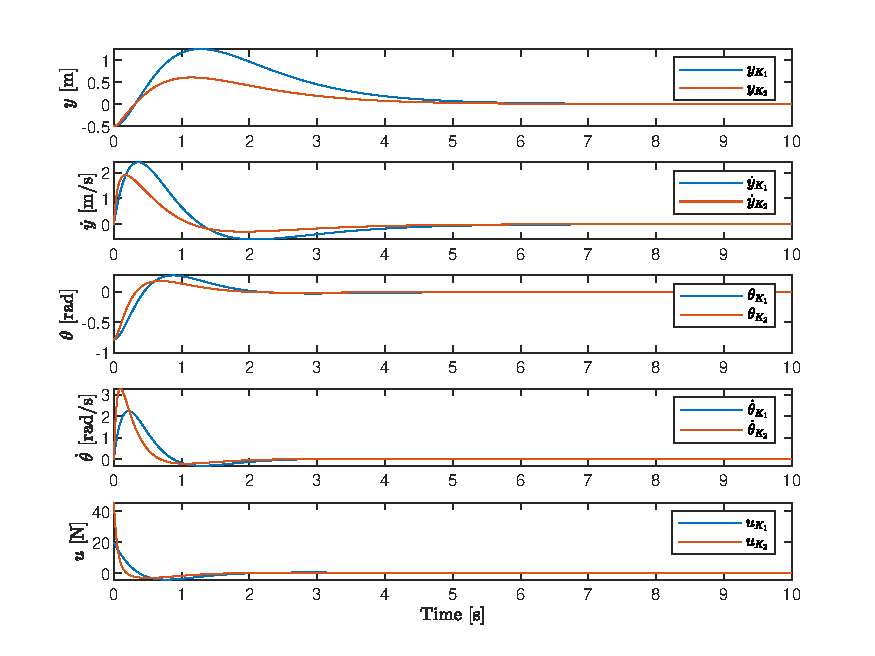
\includegraphics[0.85\textwidth]{pole_place_K1_K2_state_evolutions.pdf}
    \caption{State evolution for $K_1$ and $K_2$}
    \label{fig:state_evol_K1_K2}
\end{figure}

\subsection{Differences in transient response}
We know that our closed-loop linear system with (diagonalizable) matrix is $A_\text{cls}$ has all real eigenvalues by construction and choice above. The state evolution is therefore governed by the following (modal-decomposition) equation,

\begin{equation} \label{eqn_state_evolution}
    \vec{x}(t) = \vec{v}_1 e^{\lambda_{1}t} z_{0,1} + \vec{v}_2 e^{\lambda_{2}t} z_{0,2} + ... + \vec{v}_n e^{\lambda_{n}t} z_{0,n},
\end{equation}

where $\vec{v}_i$ are the eigenvectors of $A$. This implies that state responses are linear combinations of the eigenvectors, where the weights for each eigenvector are the exponential terms (each with a decay constant of the corresponding eigenvalue $\lambda_i$) and the coordinate some transformed initial condition $\vec{z}_0 = P^{-1}\vec{x}_0$. Here $P^{-1}$ is a coordinate transformation mapping $\vec{x}$ to $\vec{z}$.

In the pole assignment problem, we desire to assign the closed-loop system matrix as $A_\text{cls} = A+BK$ a certain set of eigenvalues, which means that the implications of equation \ref{eqn_state_evolution} are applicable here as well.
% Each eigenvalue has an associated eigenvector. Consider some eigenvector ($\vec{v}_j$), with an associated eigenvalue ($\lambda_j$), having a 0 in the $i$th component. The $i$th component of that vector would always be zero, implying the $i$th state of $\vec{x}$, $x_i$, would be unaffected by $\vec{v}_j$. 

Consider changing any one eigenvalue $\lambda_j$ in $\sigma(A_\text{cls})$. This would result in a different associated eigenvector, and hence represent $\vec{x}(t)$ in a different basis of eigenvectors. Hence, changing an eigenvalue will impact all state evolutions. This can be verified in the generated plots, where the state responses for the two different gains are not the same, meaning that each state is affected by the eigenvectors of $A_\text{cls}$. 

In this case, one eigenvalue was changed from $-4$ to $-20$. This implies a higher decay constant in the state evolution along the corresponding (changed) eigenvector which could affect all states for a given initial condition. This is visually verified in figure \ref{fig:state_evol_K1_K2} above because the system converges to zero more quickly when $K_2$ is used for the control signal over $K_1$.

\subsection{Pole assignment problem for individual state decay control}
We now discuss if it is possible to control the speed of convergence of \textit{only} individual state(s) using pole assignment. 

As discussed in the previous section, for any state $x_i$, its evolution can contain components of all modes (or eigenvectors). While we are able to control the decay rates directly, it is not necessarily true that decay rate for each state can be controlled individually, and even when this is possible for a particular system or initial condition, it is certainly not intuitive to know where to place an eigenvalues with such a constraint.

Note that the statement above is valid here because the linearized system is controllable, which was verified by checking the rank of the controllability matrix $Q_c$. However, only if the system had an uncontrollable (but asymptotically stable) subsystem, with its associated decoupled states, it would be possible to change change the speed of convergence for a state in the controllable subsystem without impacting the satisfactory speed of convergence of an uncontrollable state. 

Physically speaking, the system has only one control input that impacts all four states. Intuitively, it does not seem feasible that one control input can be manipulated such that the speed of convergence for $\theta$ is maintained. Changing the speed of convergence of $y$ will impact the speed of convergence of $\theta$ since a higher torque (resulting from higher velocity) will be applied to the pendulum, and hence it would not feasible to \textit{only} speed up the cart convergence to zero.

\section{Linear Quadradic Optimal Control}
A linear quadratic controller is a state feedback controller, $u = Kx$ such that the cost function, $J$, is minimized for a suitable gain vector $K$.
\begin{equation}
    J = \int_{0}^{\infty} \vec{x}^\intercal Q\vec{x} + \vec{u}^\intercal R\vec{u} \quad dt
\end{equation}
Here $Q$ is known as the state weight matrix and $R$ is the control cost weighted matrix  that penalizes control inputs.

For the given $Q$ and $R$ in this lab, the cost function is given by:
\begin{equation} \label{eqn_lqr}
    J = \int_{0}^{\infty} q_1x_1^2 + q_2x_3^2 + Ru^2 \quad dt
\end{equation}

Essentially, this method helps in computing $K$ such that the cost function $J$ is minimized. Although, this heuristic cost may be optimized for using a suitable $kl$, it, however, doesn't imply the best performing controller. For instance, an LQR controller will not always result in the best or needed convergence or stabilization crieteria, as seen later in this report. Note the this optimal gain vector $K$ was computed using the \textsc{MATLAB} function \texttt{lqr}.

\subsection{Impact of changing \texorpdfstring{$q_1$}{q1}}
\subsubsection{Plots}
For this subsection, $q_2$ and $R$ were fixed at $q_2 = 5$ and $R = 0.5$. Two sets of gains were computed for $q_1 = 0.1$ and $q_1 = 0.005$.

\begin{figure}[hbt!]
    \centering
    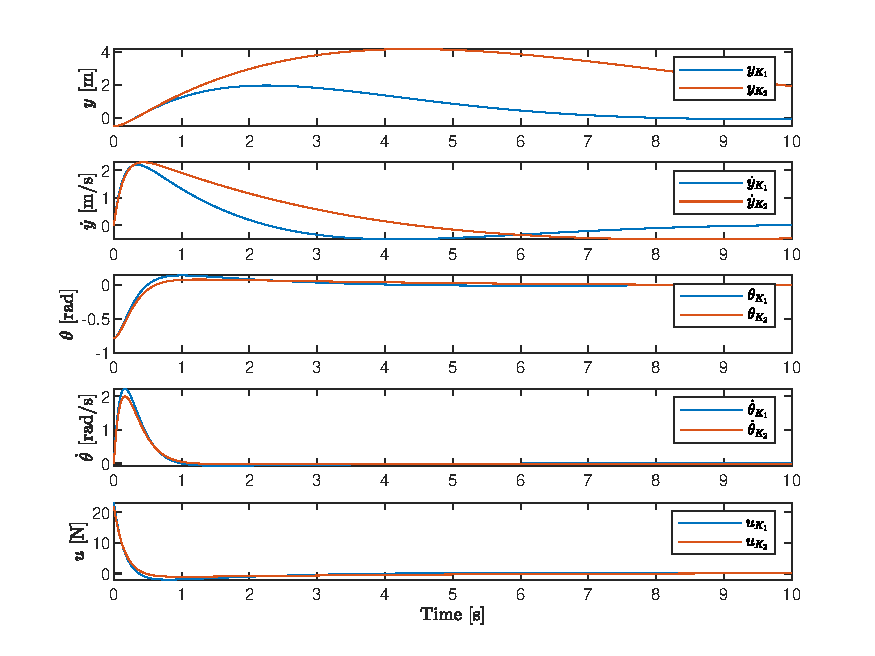
\includegraphics[0.85\textwidth]{q1_K1_K2_state_evolutions.pdf}
    \caption{State evolution for $q_1 = 0.1$ in blue and $q_1 = 0.005$ in red}
    \label{fig:q1_k1_k2_state_evolution}
\end{figure}

\subsection{Impact of changing \texorpdfstring{$q_2$}{q2}}

\subsubsection{Plots}
For this subsection, $q_1$ and $R$ were fixed at $q_1$ = 0.05 and $R$ = 0.5. Two sets of gains were computed for $q_2$ = 1 and $q_2$ = 2000.

\begin{figure}[hbt!]
    \centering
    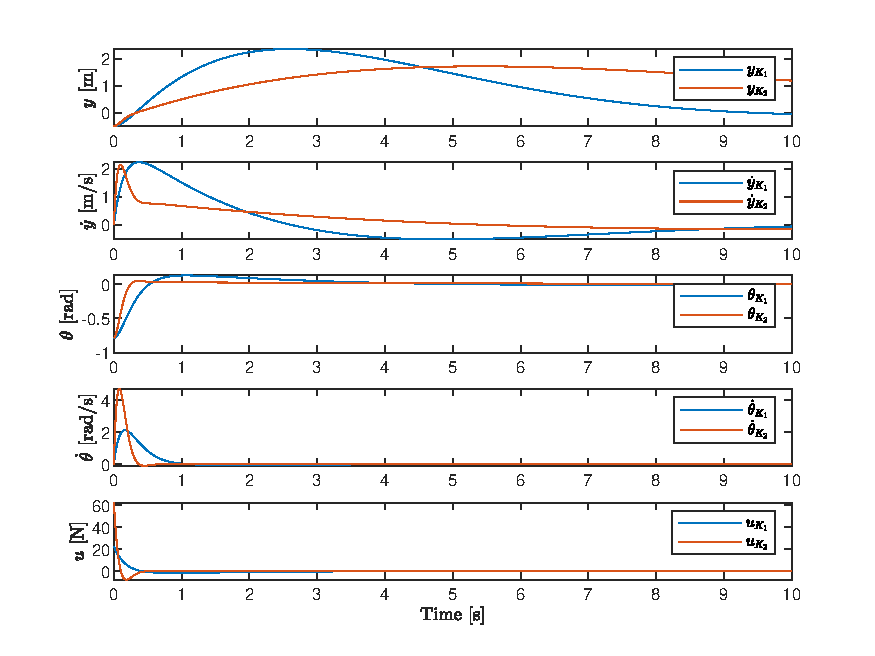
\includegraphics[0.85\textwidth]{q2_K1_K2_state_evolutions.pdf}
    \caption{State evolution for $q_2 = 1$ in blue and $q_2 = 2000$ in red}
    \label{fig:q2_k1_k2_state_evolution}
\end{figure}

\subsection{Impact of changing \texorpdfstring{$R$}{R}} \label{lqr_r_controller}

\subsubsection{Plots}
For this subsection, $q_1$ and $q_2$ were fixed at $q_1$ = 0.05 and $q_2$ = 5. Two sets of gains were computed for $R$ = 0.005 and $R$ = 10.

\begin{figure}[hbt!]
    \centering
    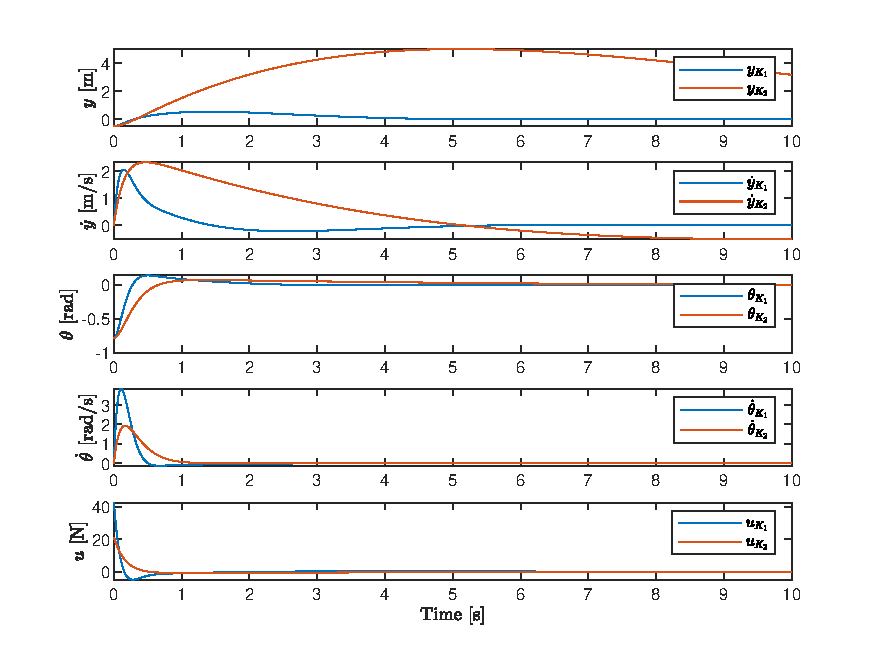
\includegraphics[0.85\textwidth]{R_K1_K2_state_evolutions.pdf}
    \caption{State evolution for $R = 0.005$ in blue and $R = 10$ in red}
    \label{fig:R_k1_k2_state_evolution}
\end{figure}

\subsection{Analysis} 
Looking at equation \ref{eqn_lqr}, $q_1, q_2 \text{ and } R$ are used to directly penalize $x_1, x_3 \text{ and } u$ respectively. The larger these values are, the more these signals are penalized. Choosing a large value for $R$ means the system is attempted to be stabilized with less energy (expensive control strategy). On the contrary, choosing a small value for $R$ means there is no penalization on the control signal (cheap control strategy). Similarly, small values for $q_1/q_2$ imply stabilization is attempted to be achieved with the least possible changes in the states, whereas large values for $q_1/q_2$ imply less concern about the changes in the states, i.e. how much the position of the cart/angle of the pendulum change to achieve equilibrium.

This can be verified in all of the graphs above. In figure \ref{fig:q1_k1_k2_state_evolution} when $q_1$ is varied, significant differences can be observed only in the $y$ and $\dot{y}$. When $K_1$ is applied (larger $q_1$), $y$ takes on a higher range of values as compared to $K_2$, indicating $K_2$ penalizes $y$ more than $K_1$. Notice changes in $\theta$ and $\dot{\theta}$ are marginally different.

Similarly, when $q_2$ is varied, in figure \ref{fig:q2_k1_k2_state_evolution}, the plots for $\theta$ and $\dot{\theta}$ are different. When $q_2$ takes on a higher value, $\theta$ is penalized relatively lesser and in fact converges to the equilibrium point more quickly than a lower value of $q_2$. Interestingly, the plots for $y$ and $\dot{y}$ are significantly different as well, and this could be attributed equations \ref{eqn_y_dot} and \ref{eqn_theta_dot}. $\dot{\theta}$ has no dependence on $y$ but $\dot{y}$ has dependence on $\theta$.

Finally, coming to figure \ref{fig:R_k1_k2_state_evolution}, it can be seen that imposing a higher value of $R$, i.e., more penalization for the input control signal ($u_{K_2}$), enforces the control signal $u$ smaller, i.e., it takes a smaller range of values.

\section{LQR controller performance on nonlinear systems}

So far, the controllers designed have been simulated on the linearized system. An interesting test for the performance of these controllers would be to simulate them on the actual non-linear system and check for convergence to the desired equilibrium point. For this section, the controller designed in section \ref{lqr_r_controller}: $R = 0.005, q_1 = 0.05, q_2 = 0.5$.

\subsection{Plots for initial condition \texorpdfstring{$(-1, 0, \pi/4, 0)$}{(−1, 0, π/4, 0)}}
The system is first tested with the $\vec{x}_0 = \rcvec{-1 & 0 & \pi/4 & 0}$. The state evolution for this is seen in figure \ref{fig:state_evol_y0}:
\begin{figure}[hbt!]
    \centering
    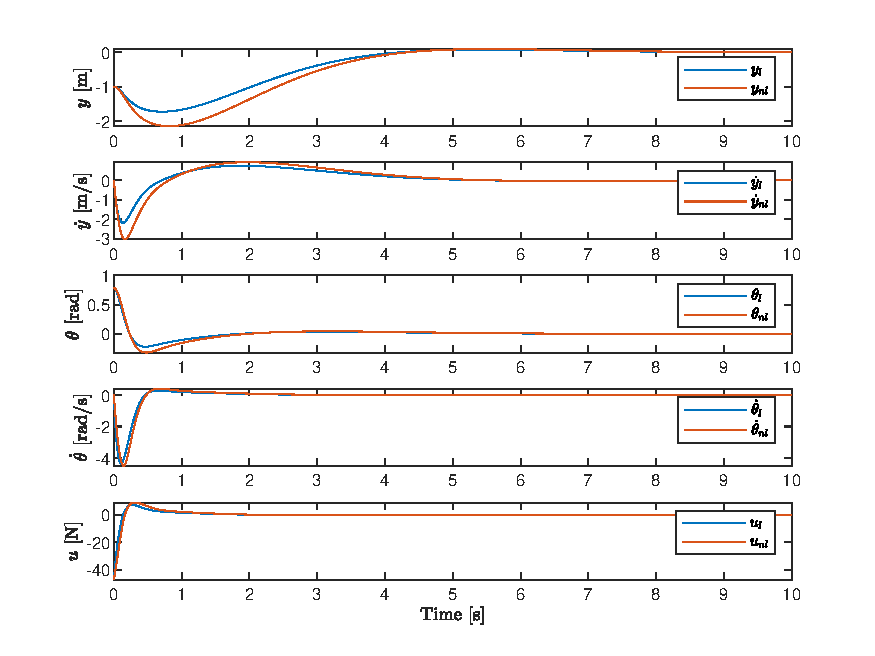
\includegraphics[0.85\textwidth]{lab3/figs/lin_nonlin_state_evolutions.pdf}
    \caption{Linear and non-linear closed-loop system state evolutions for $\vec{x}_0 = \rcvec{-1 & 0 & \pi/4 & 0}$}
    \label{fig:state_evol_y0}
\end{figure}

\subsection{Behaviour of the nonlinear system versus the linear system}
As seen in figure \ref{fig:state_evol_y0}, the lqr controller successfully converges to the equilibrium point for both the linear and non-linear systems. As an observation, it can be seen that the linear model assumes a higher restoration force, which was discussed in lab 1.

\subsection{Effect of starting farther from equilibrium}
Now, the position of the start $y$ can be further decreased until the point of no convergence is obtained. The state evolutions for decreasing $y$ is plotted in figure \ref{fig:non_lin_sys_resp_diff_y0}.

\begin{figure}[hbt!] 
    \centering
    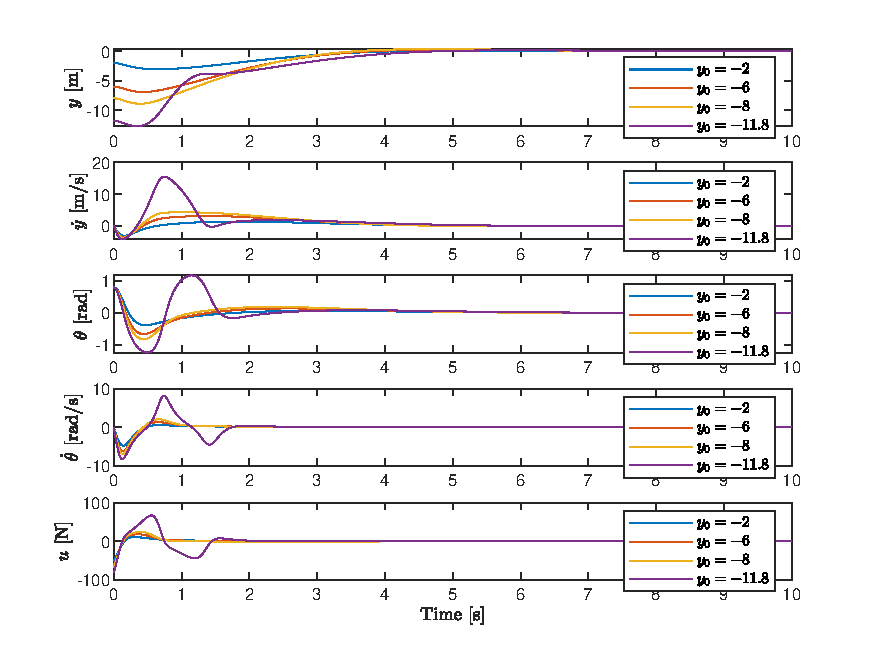
\includegraphics[0.85\textwidth]{nonlin_shiftpos_state_evolutions.pdf}
    \caption{State Evolution of the non-linear system for decreasing $y_0$}
    \label{fig:non_lin_sys_resp_diff_y0}
\end{figure}

As seen in the figure \ref{fig:non_lin_sys_resp_diff_y0}, the maximum deviations from equilibrium become larger as $y$ is decreased. The lqr controller is a more aggressive form of a proportional state feedback controller and eventually it breaks into oscillations and continues to diverge, as seen on the plots below. This was verified when $y = -11.9$, the lqr controller failed to converge to the equilibrium point (0, 0, 0, 0), as seen in figure \ref{fig:non_lin_sys_resp_unstable_y0}.

\begin{figure}[hbt!]
    \centering
    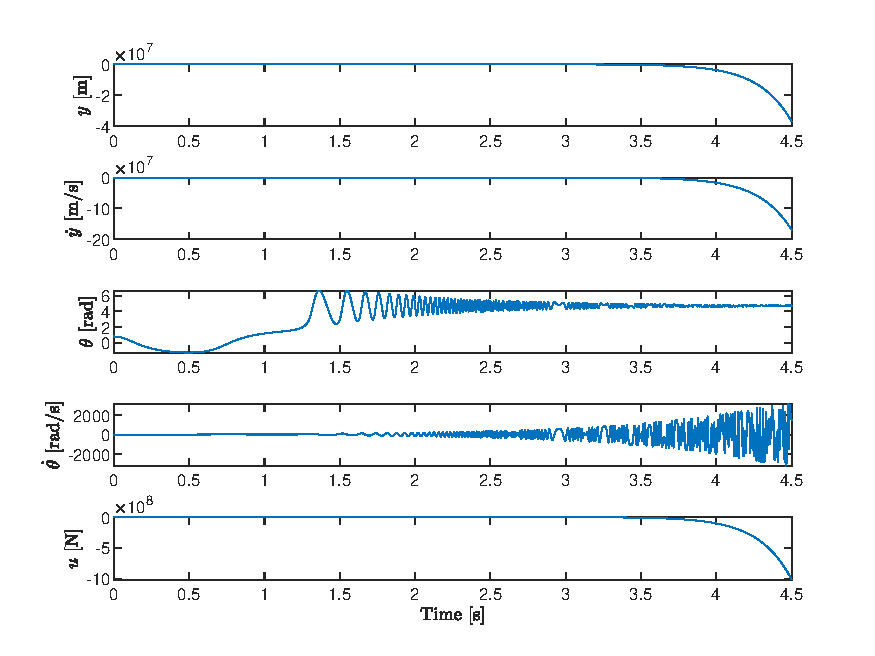
\includegraphics[0.85\textwidth]{nonlin_unstable_state_evolution.pdf}
    \caption{Unstable state evolution of the non-linear system for $y_0 = -11.9$}
    \label{fig:non_lin_sys_resp_unstable_y0}
\end{figure}

\end{document}